Upon a package request, the location of who placed the order is added to a queue. The queue is read whenever there is an available vehicle at the warehouse. Trajectories are then built from the warehouse to the destination, from the first destination to the second, and back to the warehouse. Once assigned a trajectory, the vehicle follows the reference points along the trajectory until returning to the warehouse to recharge. When in transit to the destination, the trajectory will keep the vehicle away from the no-fly-zones defined around airports and above schools. If the destination cannot be assign to a vehicle, it waits in the queue until a vehicle can serivec it. The vehicle is modeled using a point mass system driven by a controller providing reference points along the trajectory.

\begin{figure}
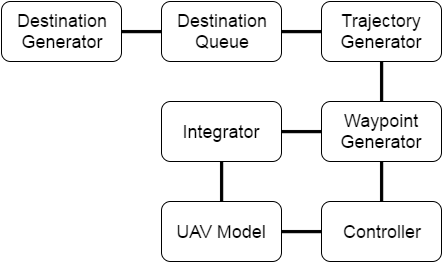
\includegraphics[width=1\linewidth]{images/TopLevelDesign.png}
\caption{Simulation Flow Chart}
\end{figure}

More complex vehicle models can be used in the simulation. The framework built provides an easy plug and play environment to interchange what model is being tested in the simulation.

